\vspace{10pt}

\minitoc
\clearpage

% % % % % % % % % % % % % % % % % % % % % % % % % % % % % % % % % % % % % % % % 
% Etat de l'Art : systèmes globaux répondant à la problématique de perception %
%	 					d'un environnement dynamique						  % 
% % % % % % % % % % % % % % % % % % % % % % % % % % % % % % % % % % % % % % % %

\section{Introduction}
On présente ici une vue d'ensemble de quelques stratégies présentes dans l'état de l'Art pour assurer à un véhicule autonome la connaissance d'un environnement dynamique. Cette problématique est largement couverte depuis quelques années, bien qu'aucune approche n'ait à notre connaissance emporté l'adhésion de tous les acteurs. Les systèmes présentés ci-dessous n'offrent ainsi pas une connaissance exhaustive de l'environnement, mais présentent chacun divers avantages, et définissent un écosystème algorithmique qui servira de référence à notre proposition. Ce sujet étant particulièrement large, toutes les techniques présentées ne sont sans doute pas couvertes dans le détail, mais on s'attachera à en faire ressortir certains des avantages et inconvénients.\\

On présente tout d'abord un ensemble de capteurs envisagés, pour répondre à notre tâche de perception de l'environnement à des fins de navigation autonome. Une observation rapide de leurs avantages et limitations nous permet ensuite d'en isoler deux types, à savoir les télémètres lasers et les solutions fondées sur la vision. Nous en présentons alors les modélisation les plus couramment utilisées, puis quelques algorithmes de l'état de l'art qui exploitent relativement directement ces modèles pour en déduire des informations utiles à la perception de l'espace et des obstacles. Nous présentons enfin quelques uns des algorithmes couramment mis en œuvre pour filtrer ces informations, et déterminer par inférence des informations qui ne sont pas directement accessibles par ces modèles. Une dernière partie est consacrée à la présentation succincte de l'approche que nous proposons, et qui sera amplement développée dans les prochaines parties. 

\section{Différents capteurs possibles} \label{sec:ch2_capteurs}
%\subsection{Capteurs actifs et passifs}
%On segmente ici les capteurs couramment utilisés en deux catégories arbitraires, qui rendent compte de la différence fondamentale entre les informations perçues : les capteurs "actifs" et %les capteurs "passifs". Dans notre segmentation, les capteurs actifs émettent une onde (acoustique ou électromagnétique) qui va permettre de "sonder" l'espace. Les capteurs que l'on appelle %"passifs" n'émettent, comme leur nom l'indique, aucune onde de quelque nature que ce soit, mais captent une onde présente dans l'environnement. Ces différences dans le mode d'action ont des %conséquences sur les informations perçues : les premiers acquièrent généralement l'espace libre dans une direction donnée, tandis que les seconds perçoivent une projection de l'environnement %selon un axe. Ces différences peuvent être directement reliées au mode de représentation de l'information choisi (insérer référence), mais cela n'est pas nécessairement le cas.

\subsection{Comparaison capteurs et besoins}
De nombreux capteurs sont envisageables à des fins de perception, aux avantages divers et parfois complémentaires. En faire une étude détaillée n'est pas l'objet de ce manuscrit, mais ce paragraphe est consacré à une brève revue de détails, afin de sélectionner les capteurs les plus à même de répondre à nos besoins. Le tableau \ref{tab:ch2_Comparaison_capteurs} offre une vue synthétique de l'adéquation des capteurs envisageables avec nos besoins, et peut être complété par les remarques suivantes :
\begin{itemize}
\item{\emph{Ultrasons:\\}}
Ces capteurs permettent une mesure de l'espace libre, mais leur très faible portée et précision limitent les informations accessibles.\\

\item{\emph{Différents télémètres laser:\\}}
On dissocie arbitrairement dans \ref{tab:ch2_Comparaison_capteurs} les télémètres laser ne comportant que quelques couches et une ouverture limitée et les télémètres de type \og Velodyne\fg{}. Ces derniers seront souvent pris comme référence par la suite, leur utilisation étant devenue courante pour des applications de cartographie ou de navigation autonome de véhicule. Ils sont constitués d'un alignement de télémètres pivotant autour d'un axe, autorisant une couverture angulaire de 360$^\circ$ par 60$^\circ$, et fournissant des centaines de milliers de points par seconde. La densité d'informations plus faible fournie par les premiers rend par exemple difficile la détection et le suivi d'objets mobiles (\cite{Wang2007, Gate2009}), ou encore la perception de l'espace navigable.\\

\item{\emph{Mono et multi-caméras:\\}}
On dissocie de même les solutions mono et multi-caméras, au vu de l'état de l'art dans leurs domaines respectifs (la perception d'un volume par une solution mono-caméra immobile est par exemple délicate). L'évaluation de la portée des solutions visuelles est délicate, selon la nature de l'information exploitée. La reconnaissance de forme ou la détection d'obstacles peuvent ainsi être typiquement réalisées à de grandes distances (\cite{Labayrade2002}), tandis que le positionnement dans l'espace est en général plus délicat. Ces performances sont par ailleurs dépendantes de la résolution du système utilisé, mais aussi de la disposition relative des caméras dans le cas de systèmes de stéréo-vision (un écartement plus important augmentant la précision de positionnement à grande distance). \\

\item{\emph{Radar:\\}}
La portée très importante (environ 200 mètres) et le faible coût des radars embarqués rend ce capteur d'ores et déjà populaire dans l'industrie automobile, mais il est pénalisé dans notre comparaison par sa faible résolution spatiale, et son ouverture angulaire limitée. De nombreuses études font cependant état de développements avancés (notamment dans la détection de piétons, voir par exemple Vivet \cite{Vivet, Vivet2013} ou Milch \cite{Milch2001}). L'ouverture angulaire limitée peut notamment être compensée par une structure tournante, comme c'est le cas pour les télémètres laser, bien que cette solution soit certainement industriellement complexe.\\

\item{\emph{Caméras de profondeur:\\}}
Les caméras dites \og 3D\fg{} (utilisant en général de la lumière structurée ou une mesure du temps de vol) n'ont pour l'instant pas réellement d'utilisation possible à l'extérieur, et ne sont donc pas envisageables pour notre application. De nouveaux dispositifs sont cependant présentés depuis quelques années, tirant profit de déformations optiques volontaires ou d'un réseau de micro-lentilles par exemple, et leur usage pourrait se généraliser dans un futur proche.\\

\item{\emph{Prix de revient:\\}}
Le prix des capteurs n'entre pas en compte dans ce tableau, qui se veut le plus général possible. Les coûts des solutions présentées diffèrent cependant grandement, que ce soit au niveau du capteur ou des traitements informatiques afférents.\\
\end{itemize}

\begin{figure} 
	\centerline{
		\includegraphics[width=1\textwidth]{Chapter2/graphics/sensor_needs.png}
		}
	\caption{Représentation approximative des propriétés respectives de différents types de capteurs. Les solutions présentes sont classées par leur couleur, du vert vif (point fort) au rouge vif (point faible). Une couleur moins saturée décrit une caractéristique positive ou négative moins marquée.}
	\label{tab:ch2_Comparaison_capteurs}
\end{figure}

On constate aisément au vu du tableau \ref{tab:ch2_Comparaison_capteurs} que les capteurs de type \og télémètre laser\fg{} et \og vision\fg{} sont \textit{a priori} les plus intéressants pour un tel usage. Ce constat n'est par ailleurs pas étonnant au vu de la littérature sur le sujet, qui se concentre effectivement sur ces moyens de mesure. La suite du manuscrit est donc plus particulièrement consacrée à ces deux moyens de perception.

\subsection{Modèles de capteurs}
Les informations issues d'un capteur doivent nécessairement être interprétées, pour prendre en compte son mode d'acquisition, ou les incertitudes qui y sont associées. Les capteurs perceptifs illustrent en effet différentes facettes de l'environnement, observant par exemple l'occupation selon une direction donnée ou la projection du champ électromagnétique sur un plan. Ces spécificités sont prises en compte par un modèle de capteur, description algorithmique qui permet de traduire les informations obtenues en sortie de capteur en une représentation plus abstraite. Le modèle de capteur fait donc le lien entre la mesure physique effectuée par celui-ci et les informations qui en découlent. Les modèles de capteur les plus couramment associés aux télémètres laser et à la vision sont présentés dans les sections suivantes.

\subsubsection{Télémètre laser} \label{sec:ch2_Modèle_laser}
Le télémètre laser est un capteur actif, en cela qu'il émet une onde qui \og sonde\fg{} l'espace, et qui permet de déterminer la distance au premier point d'impact (souvent par mesure du temps de vol, mais d'autres techniques, notamment fondées sur un déphasage de l'onde réfléchie ou sur l'effet Doppler sont possibles). Il fournit, de part la localisation de ce point, l'information paradoxale de l'espace libre entre le point d'émission et celui ci. Le modèle de capteur doit rendre compte de cette observation, et une approche fréquente consiste à le définir en termes de probabilité d'occupation. Celle-ci est en général négligeable entre le point d'émission et le point d'impact relevé, maximale au niveau du point d'impact, puis prolongée à son niveau maximal ou décroissante selon les besoins. La localisation du point d'impact peut être modélisée par une probabilité de présence continue, par exemple gaussienne, rendant compte de la stochastique du capteur, ou par une série de valeurs discrètes, arbitraires, rendant parfois compte de différents besoins des algorithmes en aval dans le processus de traitement. On en présente quelques exemples sur la Figure \ref{fig:ch2_laser_model}.

\begin{figure}[h]
\centering{
	\includegraphics[width=0.9\textwidth]{Chapter2/graphics/laser_model.png}
	\caption{Exemples de différentes modélisations d'un télémètre laser, définissant la probabilité d'occupation en fonction de la distance au point d'émission et au point d'impact. La courbe bleue représente une probabilité d'occupation continue, Gaussienne. Les courbes rouges et vertes représentent un modèle discret couramment utilisés dans les représentations dites de \og grilles d'occupation\fg{}, et considèrent différemment la probabilité d'occupation de la partie occultée par le point d'impact.}
	\label{fig:ch2_laser_model}
	}
\end{figure}

La généralisation des modèles discrets dans le cas de télémètres lasers à balayage conduit souvent à une représentation dans le plan de rotation, dans laquelle la probabilité d'occupation de l'espace est échantillonnée selon une grille. On en présente un exemple dans la Figure \ref{fig:ch2_laser_grid}, dont la scène est tirée des acquisitions du projet LOVe de protection des vulnérables sur la route.

\begin{figure}[h]
	\begin{center}
		\begin{subfigure}{0.48\textwidth}
			\includegraphics[width=\textwidth]{Chapter2/graphics/laser_occupancy_grid_pict.png} 
			\caption{Vue de la caméra}
		\end{subfigure}	
		~	
		\begin{subfigure}{0.48\textwidth}
			\includegraphics[width=\textwidth]{Chapter2/graphics/laser_occupancy_grid.png} 
			\caption{Application d'un modèle (\ref{fig:ch2_laser_model}) aux acquisitions d'un télémètre laser.}
		\end{subfigure}
		
		\caption{Exemple de modèle d'un télémètre laser à balayage : représentation sous la forme d'une grille d'occupation. Dans cette représentation le capteur est situé au plus bas de la grille, pointant vers le haut. La probabilité d'occupation est représentée en niveaux de gris}
		\label{fig:ch2_laser_grid}
	\end{center}
\end{figure}

On constate aisément que ce modèle autorise une détection immédiate des possibles obstacles statiques ou dynamiques, par un simple critère de proximité. Les informations extraites du capteur sont cependant minimales dans ce cas (pas de segmentation, de classification, de dynamique par exemple), et l'utilisation d'algorithmes d'inférence (voir \ref{sec:ch2_perception_spécifique} et \ref{sec:ch2_Algo_total}) est le plus souvent préférable. \\

Il n'est par ailleurs pas indispensable d'utiliser une vision probabiliste et basée sur l'occupation pour exploiter les données d'un télémètre laser. L'apparition de capteurs très denses et en trois dimensions (de type \textit{Velodyne}) a rendu possible une exploitation plus directe des mesures de points d'impact, pas nécessairement basée sur le modèle précédent.

\subsubsection{Vision}
On restreint les dispositifs de vision décrits ici à un ensemble optique accolé à un capteur d'imagerie, bien que d'autres approches soient certainement possibles sous cette dénomination. 

\paragraph{Modèle sténopé\\}
Le modèle dit \og sténopé\fg{}, du nom du dispositif optique minimal permettant l'imagerie d'une scène sur un capteur via un simple trou dans une surface opaque, est le plus couramment utilisé pour modéliser le processus d'acquisition d'images à partir d'une scène en trois dimensions. On considère dans l'équation \ref{eq:ch2_modèle_sténopé} les coordonnées ${u,v}$ dans le plan image, et ${X,Y,Z}$ dans le repère monde. L'orientation de ces repères est la suivante :
\begin{itemize}
	\item{} $u$ et $x$ sont parallèles et orientés dans le même sens, de même que $v$ et $y$.\\
	\item{} $z$ complète $x$ et $y$ pour en faire un repère orthonormé, et est orienté vers le fond de la scène.\\
	\item{}	$f$ est la focale de l'optique, c'est à dire la distance entre le plan optique et le plan de convergence d'un front d'onde provenant d'une source située à l'infini. L'équation suivante s'obtient aisément en considérant un système optique simplifié (une seule lentille de focale connue) et des observations géométriques.\\
\end{itemize}

Les coordonnées $u_0$ et $v_0$ décrivent les distances dans le plan image entre l'origine du repère, qui peut être choisie arbitrairement (par exemple en haut à gauche de l'image dans le cas d'un adressage informatique), et l'intersection de l'axe optique et du plan image. Une représentation de ce modèle est visible sur la figure \ref{fig:ch2_modèle_sténopé}.

\begin{figure}[h]
	\begin{center}
		\includegraphics[width=0.7\textwidth]{Chapter2/graphics/pinhole_model.png}
		\caption{Illustration du modèle sténopé}
		\label{fig:ch2_modèle_sténopé}
	\end{center}
\end{figure}

\begin{equation} \label{eq:ch2_modèle_sténopé}
	\begin{array}{|c}
		u\\
		v\\
	\end{array}
= 
	\begin{array}{|c}
		u_0 + f \cdot \frac{X}{Z}\\
		v_0 + f \cdot \frac{Y}{Z}\\
	\end{array}
\end{equation}

La transformation décrite n'est pas bijective, c'est à dire que la connaissance de la position dans l'espace d'un objet permet d'en déduire sa projection sur le plan image, mais que le processus inverse n'est pas déterminé. La position dans l'espace d'un point présent dans le plan image est déterminée à un degré de liberté près, ce qui se matérialise par une ligne dans l'espace sur laquelle ce point peut se trouver.\\

Ce modèle est par ailleurs une représentation simplifiée du processus d'imagerie, mais il reste très largement utilisé et souvent suffisamment performant. L'approximation d'une projection parfaite de l'image sur un plan n'est pas respectée pour les caméras dotées d'un très grand angle de prise de vue, et d'autres modèles peuvent alors être introduits (projection sur une sphère notamment), qui ne seront pas détaillés ici. Il est par ailleurs possible de modéliser les erreurs optiques distordant l'image projetée par des polynômes simplifiés, décrivant la projection d'une droite du repère monde dans le plan image. Cette correction est souvent relativement grossière, les applications à base de vision dans le domaine de la robotique étant empiriquement peu sensibles aux erreurs de rectilinéarité.

\paragraph{Stéréo-vision\\} \label{sec:ch2_Modèle Stéréovision}
Un dispositif de stéréo-vision combine deux caméras dont les positions et orientations relatives sont connues. Le modèle \og sténopé\fg{} peut à nouveau être mis à profit dans ce cas de figure, et la connaissance de la position d'un élément de l'espace dans deux plans image distincts permet cette fois de définir un modèle global bijectif. On peut en effet reprendre les calculs \ref{eq:ch2_modèle_sténopé}, et les développer dans le cas d'une projection sur les plans image $P_1$ et $P_2$, dont on connaît les positions relatives. Il faut dans ce cas tenir compte de l'origine distincte des deux repères utilisés pour la projection. Dans un cas quelconque, les repères des deux caméras diffèrent d'une transformation rigide, composée d'une rotation et d'une translation, comme illustré dans la figure \ref{fig:ch2_stereo_quelconque}. \\
On a vu que l'antécédent d'un point du plan image par l'équation du modèle sténopé (\ref{eq:ch2_modèle_sténopé}) était une droite. On définit dans ce cas la droite épipolaire liée au point $M$ comme l'image par le capteur $C_2$ de la droite antécédente de la projection du point $M$ sur le capteur $C_1$. Cette droite est importante lors de la recherche dans le plan $P_2$ de la projection du point $M$, lorsque celle-ci est déjà connue dans le plan $P_1$. Le point $M$ imagé par le capteur $C_2$ peut alors être recherché le long de la droite épipolaire uniquement.\\

\begin{figure}[h]
		\begin{center}
			\includegraphics[width=0.7\textwidth]{Chapter2/graphics/stereo_model_random.png}
			\caption{Système de stéréo-vision quelconque. Les angles sont exagérés par rapport à un système typique, pour les besoins de l'illustration.}
			\label{fig:ch2_stereo_quelconque}
		\end{center}
\end{figure}

L'utilisation de l'équation \ref{eq:ch2_modèle_sténopé} appliquée à chacune des caméras, et exprimée dans un même repère, nécessite alors l'usage d'une matrice de rotation et d'un vecteur de translation. Il est cependant possible de grandement simplifier les calculs par une opération dite de \og rectification\fg{}, qui permet de se placer dans le cas où les repères des deux plan image sont reliés par une unique opération de translation. Cette correction peut être effectuée sur un système de stéréo-vision dont les caméras sont approximativement alignées, au prix d'une réduction de la surface imagée par chaque caméra. Elle implique de déterminer préalablement les paramètres géométriques reliant les deux systèmes de coordonnées. Afin de simplifier les calculs de disparité, c'est à dire de la différence de position d'un même élément image dans les deux plan image, il est courant de corriger les images afin de se ramener à une translation le long du vecteur $\arrowvert{u}$ entre les deux plan image.

\begin{figure}[h]
	\begin{center}
		\includegraphics[width=0.7\textwidth]{Chapter2/graphics/stereo_model_rectified.png}
		\caption{Système de stéréo-vision rectifié}
		\label{fig:ch2_stereo_rectifié}
	\end{center}
\end{figure}

Les équations décrivant la relation entre le référentiel \og monde\fg{} et les deux plan image peuvent alors s'écrire relativement simplement (équation \ref{eq:ch2_modèle_stéréo}).

\begin{align} \label{eq:ch2_modèle_stéréo} 
	\begin{split}
		\begin{array}{|c}
		u_1\\
		v_1\\
		\end{array}	
		&=
		\begin{array}{|c}
		{u_0}_1 + f_1 \cdot \frac{X - X_1}{Z - Z_1}\\
		{v_0}_1 + f_1 \cdot \frac{Y - Y_1}{Z - Z_1}\\
		\end{array}	\\ \\
		\begin{array}{|c}
			u_2\\
			v_2\\
		\end{array}
		&= 
		\begin{array}{|c}
			{u_0}_2 + f_2 \cdot \frac{X - X_2}{Z - Z_2}\\
			{v_0}_2 + f_2 \cdot \frac{Y - Y_2}{Z - Z_2}\\
		\end{array}
	\end{split}
\end{align}

Si l'on suppose maintenant que l'origine de chacun des repères image est définie de la même façon (${u_0}_1 = {u_0}_2$, ${v_0}_1 = {v_0}_2$), et que les focales des systèmes optiques sont les mêmes ($f_1 = f_2$), on peut utiliser la rectification pour simplifier l'équation \ref{eq:ch2_modèle_stéréo}. Les repères des deux caméras peuvent être représentés par un unique repère, dans lequel $Y_1 = Y_2 = Y_C$, $Z_1 = Z_2 = Z_C$, et $X_2 = X_1 + b$ (avec $b$ l'écartement entre les deux centres optiques des caméras $C_1$ et $C_2$, nommée \textit{baseline} dans la littérature anglophone). On obtient finalement les équations bien connues d'un système de stéréo-vision, reliant le repère monde au repère unifié des deux caméras (équation \ref{eq:ch2_stereo_equations}).

\begin{align} \label{eq:ch2_stereo_equations}
	\begin{split}
		z& = \frac{f * b}{d}	\\
		y& = \frac{(v - v_0) * z} {f}	\\
		x& = \frac{(u - u_0) * z} {f}
	\end{split}
\end{align}

Ce calcul peut alors être exploité pour connaître la position de tout ou partie des éléments imagés, exception faite des éléments visibles sur une seule des deux caméras. Dans la perspective d'une détection d'obstacles, on peut alors choisir de se concentrer sur les informations présentes dans la carte de disparité (homogène à une ligne de vue dans la direction de chacun des pixels considérés), comme illustré sur la figure \ref{fig:ch2_disparity_map}. Il est également possible de se fonctionner directement dans le repère \og monde\fg{}, à partir des coordonnées (x, y, z).\\

\begin{figure}[h]
	\begin{center}
		\begin{subfigure}{0.48\textwidth}
			\includegraphics[width=\textwidth]{Chapter3/graphics/OF_Farneback_RAW.png} 
			\caption{Une des deux images sources.}
		\end{subfigure}	
		~	
		\begin{subfigure}{0.48\textwidth}
			\includegraphics[width=\textwidth]{Chapter2/graphics/dense_disparity.png} 
			\caption{Carte de disparité.}
		\end{subfigure}
		
		\caption{Exemple de carte de disparité obtenue par la méthode ELAS (Geiger,\cite{Geiger}). La disparité est représentée par une valeur en niveaux de gris}	
		 \label{fig:ch2_disparity_map}
	\end{center}
\end{figure}

Une limite de ce modèle réside dans le bruit associé à la localisation dans l'espace, fortement anisotrope pour une distance grande devant la \textit{baseline} (voir par exemple \cite{Blostein1987}, \cite{Demirdjian2001} ou \cite{Sibley2007}, \cite{Lenz2011}). Ce bruit peut être modélisé, si l'on néglige les erreurs de calibration optique et géométrique du dispositif, par les équations suivantes : 

\begin{itemize}
	\item La position d'un même point est déterminé sur les deux plans image avec la dispersion $\delta$, que l'on suppose isotrope dans le plan image. Cette dispersion peut être liée à l'échantillonnage de l'image sur ses deux axes, mais aussi à la procédure d'identification du point, par exemple lors d'une corrélation (la largeur du pic de corrélation n'est pas nulle, et introduit donc une erreur possible de positionnement).\\
	
	\item Le calcul de l'erreur de positionnement d'un point dans l'espace consécutif à une erreur de positionnement $\delta$ dans le plan image (pour un dispositif rectifié) s'écrit :
	\begin{align}
		\begin{split}
			\delta_z &= \frac{\delta \cdot f \cdot b}{d^2} \\
			\delta_x &= \frac{\delta \cdot (u - u_0) \cdot b}{d^2} \\
			\delta_y &= \frac{\delta \cdot (v - v_0) \cdot b}{d^2} \\
		\end{split}
	\end{align}
\end{itemize}

On constate aisément que l'erreur de positionnement est dépendante de la position du point par rapport à l'axe optique, et de l'éloignement du point par rapport au plan image. Ce bruit de changement de repère est par exemple illustré par la Figure \ref{fig:bruit_disparité}, tirée de la publication de Lenz et al \cite{Lenz2011}.

\begin{figure}
	\centering{
		\includegraphics[width=0.6\textwidth]{Chapter2/graphics/noise_disparity.png}
	}
	\caption{Illustration du bruit lors du changement de repère (image -> monde), tirée de \cite{Lenz2011}}
	\label{fig:bruit_disparité}
\end{figure}

\subsection{Capteur retenu dans le cadre de la méthode proposée} \label{sec:ch2_capteur_retenu}
Nous avons choisi de nous concentrer sur l'usage d'un dispositif de stéréo-vision, bien qu'un travail préliminaire en début de thèse ait été consacré à l'usage d'un télémètre laser (voir \ref{sec:ch5_Bayésien_2D}). Ce travail préliminaire a mis en avant la difficulté d'estimation de la vitesse des éléments de la scène avec un tel capteur, et nous avons pensé que l'usage de la vision était intéressant dans ce cadre, parallèlement à d'autres avantages propres (coût de mise en œuvre, usages variés -reconnaissance de personnes, de panneaux, etc..-). L'état de l'art dans le domaine de l'association dans le temps d'éléments visuels d'une scène est en effet important, ce qui autorise alors une estimation de la vitesse relative des éléments de la scène. Cette tâche est toujours délicate avec un capteur télémétrique, et demeure une problématique de recherche actuelle.
La nécessité d'avoir deux caméras peut être un handicap par rapport aux dispositifs mono-caméra, qui est souvent mis en avant dans la littérature. Les informations disponibles sont cependant plus importantes dans ce cadre, et comme nous l'avons montré dans ce travail, autorisent des usages nouveaux. La reconstruction d'environnement dense, la détection et le suivi d'objets mobiles, la perception d'un environnement en trois dimensions par un dispositif à l'arrêt sont autant de tâches accessibles à un système stéréo-vision, et plus difficilement appréhendable par les systèmes mono-caméra. 

\section{Différents types de représentations}
Indépendamment des capteurs utilisés, les informations collectées par le capteur ou par le mécanisme d'accumulation mis en place peuvent utiliser différentes représentations. Celles-ci sont liées aux algorithmes d'inférence ou de fusion de données utilisés, et peuvent avoir des avantages spécifiques. Elles ne sont pas nécessairement exclusives, plusieurs représentations étant parfois utilisées parallèlement.

\subsection{Représentation des attributs physiques}
Les caractéristiques physiques déterminées par le capteur, ou par inférence, peuvent être soumises à différentes représentations. On peut mettre en avant deux approches, très différentes par leur principe et par leurs conséquences sur l'accumulation de l'information. De manière arbitraire, on classe les approches suivantes selon l'élément clef du référencement des observations : l'espace, ou le temps. On se concentre dans le premier cas sur une information, dont on veut connaître la valeur en tout point de l'espace, par exemple la probabilité d'occupation. Dans le second cas, on se concentre sur l'évolution dans le temps de points de mesure, par exemple la position d'un objet initialement détecté.\\

\subsubsection{Représentation dense dans l'espace}
On peut tout d'abord présenter les représentations liées à la connaissance de l'espace, dans lesquelles les informations sont cumulées de part leur position. On cherche ici à connaître l'ensemble du champ de valeur autour du véhicule, qu'il s'agisse de l'occupation, de la vitesse, ou d'autres caractéristiques (navigabilité, etc). Les informations sont dans ce cas placées sur une \og grille\fg{}, échantillonnage régulier ou non de l'espace, tel qu'initialement proposé par Moravec et Elfes (\cite{Moravec1985, Elfes1989a,Elfes1987}). Une représentation d'une telle grille d'occupation, telle qu'obtenue par Moravec et Elfes dans leur publication initiale, et visible sur la figure \ref{fig:ch2_grille_occupation}. \\

Les lois de mise à jour d'une telle représentation peuvent prendre des formes différentes, et intègrent souvent une inférence Bayésienne. Plus récemment, la théorie des croyances, introduite par Dempster et Shafer (\cite{Dempster1967}), est également fréquemment utilisée (voir par exemple Moras \textit{et al.}\cite{Moras2011a}). Cette représentation a l'avantage de la densité dans l'espace, et est souvent très appropriée aux moyens de calculs informatiques, de part sa régularité. \\
On suppose cependant le plus souvent dans cette représentation que le système peut être modélisé par une chaîne de Markov d'ordre 1, c'est-à-dire que toutes les informations permettant de prédire l'état futur sont contenues dans l'observation précédente. La considération d'ordres supérieurs augmente en effet très rapidement les coûts calculatoires dans le cas d'une représentation \og dense\fg{} comme celle-ci, au point d'être en pratique impossible. L'appariement des mesures d'une itération sur l'autre n'est en revanche pas nécessaire dans cette approche, ce qui en fait une représentation couramment utilisée pour les capteurs pour lesquels cette étape est délicate (télémètres lasers par exemple). 

\begin{figure}
	\centering{
		\includegraphics[width=0.6\textwidth]{Chapter2/graphics/moravec_elfes_occupancy_grid.png}
	}
	\caption{Grille d'occupation obtenue par un capteur sonar, tirée de la publication séminale de Moravec et Elfes \cite{Moravec1985}. Les positions du capteur lors des différentes acquisitions sont représentées par des cercles. La probabilité d'occupation est illustrée par le symbole \og X\fg{}, selon sa largeur. Une probabilité d'occupation inconnue est représentée par le symbole \og .\fg{}.}
	\label{fig:ch2_grille_occupation}
\end{figure}

\subsubsection{Représentation dense dans le temps}
Par opposition à l'approche spatiale basée sur des grilles présentées précédemment, il est possible d'adopter une approche complémentaire, qui prend en compte les observations concernant une même entité au fil du temps. Cette approche suppose un appariement des observations, par exemple sur des critères spatiaux ou visuels. Cette étape peut être délicate, mais divers cadres probabilistes existent (voir par exemple la section \ref{sec:ch5_GMPHD}). Il est possible dans cette représentation d'envisager une modélisation prenant un important historique de mesures en compte, même si cette possibilité est rarement exploitée, du fait de coûts calculatoires rapidement rédhibitoires. La faible densité des informations (limitées aux observations) peut rendre cette solution intéressante dans un cas où les capacités de calcul sont limitées. \\
Un exemple d'une telle représentation est visible sur la figure \ref{fig:ch2_suivi_temps_epars}, tirée des travaux de Schindler et al. \cite{Schindler2010} à des fins illustratives uniquement. Les observations sont éparses dans l'espace, et correspondent à des candidats possibles pour une détection et un suivi de piétons (\textit{a}). Les observations sont associées dans le temps (\textit{b}), et génèrent alors une trajectoire dense dans le temps (chaque pas de temps est associé à une position dans l'espace). Plusieurs cibles peuvent être suivies simultanément, la connaissance d'une trajectoire passée permettant d'envisager plus précisément les associations futures (\textit{c} et \textit{d})

\begin{figure}
	\centering{
		\includegraphics[width=0.8\textwidth]{Chapter2/graphics/schindler_pedestrian_tracking.png}
	}
	\caption{Suivi de cibles dans le temps, à partir d'observations éparses dans l'espace. Illustration tirée de \cite{Schindler2010}}
	\label{fig:ch2_suivi_temps_epars}
\end{figure}

\subsection{Représentation ensembliste, par connexité}
Il est parfois bénéfique d'ajouter aux connaissances précédemment décrites celle de liens existant entre plusieurs entités observées. Ces liens peuvent, par exemple, être temporels (le même objet est visible sur plusieurs acquisitions, à des positions potentiellement différentes) ou spatiaux (acquisitions liées par leur proximité géographique). Ces liens décrivent une topologie particulière, un graphe, dont l'exploitation est souvent primordiale dans un contexte de rapidité d'exécution et de robustesse.\\
De nombreuses publications récentes tirent profit de ces organisations topologiques, que ce soit pour exploiter les fermetures de boucles (passages répétés dans le même environnement, source d'information pour un système SLAM, voir par exemple FrameSLAM \cite{Konolige2008} - Slam visuel par optimisation - , GraphSLAM \cite{Thrun2006a} - SLAM laser à grande échelle-, Strasdat \cite{Strasdat} - pour une extension d'un SLAM visuel à base d'EKF prenant en compte les fermetures de boucles -) ; ou pour accélérer la localisation dans un environnement préalablement cartographié (voir par exemple Meilland \cite{Meilland2011} pour un rapprochement d'une observation avec des sphères d'images et de cartes de profondeur, ou Sinha \cite{Sinha2012} pour une relocalisation au sein d'un environnement modélisé à partir de \og Structure From Motion\fg{} (SFM)). Une illustration de la représentation utilisée par FrameSLAM est présente sur la figure \ref{fig:ch2_connexité}.

\begin{figure}
	\centering{
		\includegraphics[scale=0.5]{Chapter2/graphics/frame_slam.png}
		\caption{Exemple de représentation par connexité, tirée de l'article \cite{Konolige2008} présentant FrameSLAM (Konolige et al.). Les acquisitions se font le long de la trajectoire bleu foncé, chaque acquisition étant représentée par un cercle rouge. Les segments rouges lient les acquisitions présentant des éléments en commun malgré une grande séparation temporelle.}
		\label{fig:ch2_connexité}
	}
\end{figure}

\subsection{Représentation paramétrique : introduction d'un \textit{prior}} \label{sec:ch2_représentation_paramétrique} % Paramétrique ?
L'environnement dans lequel les moyens de mesure évoluent est souvent connu, et il peut être intéressant d'en tirer profit dans la représentation qui en est faite. Cette notion s'appelle un \og prior\fg{} dans le domaine des probabilités, a savoir l'exploitation d'une connaissance a priori de certains éléments auxquels des propriétés peuvent être associés une fois leur identification effectuée. Ces propriétés connues peuvent concerner plusieurs domaines, par exemple (et pas exclusivement) : 
\begin{itemize}
	\item {\textit{Les caractéristiques spatiales : }\\}
	l'environnement rencontré peut souvent être décrit par des primitives (lignes droites, courbes paramétrées, etc..), ou par un jeu de formes de base. Ce \textit{prior} peut notamment améliorer la précision et la robustesse du positionnement et de la cartographie, ou simplifier son enregistrement. Moutarlier et Chatila proposent ainsi l'utilisation de lignes droites en deux dimensions pour représenter un environnement plan, et en déduire le mouvement d'un robot à partir d'acquisitions d'un télémètre laser (\cite{Moutarlier1990a}). Cette représentation peut simplifier l'accumulation des connaissances, en réduisant les degrés de liberté des informations conservées, mais aussi rendre un algorithme plus robuste au bruit. Le processus d'association des mesures à un modèle peut en effet tolérer des erreurs, tandis que la précision du modèle obtenu est ensuite fonction du nombre de points de mesure mis à contribution. On peut de ce fait obtenir les paramètres relativement précis d'un modèle à partir d'acquisitions bruitées. L'appariement des acquisitions successives est également rendu plus facile par cette modélisation, que ce soit pour estimer le mouvement du véhicule, ou pour estimer le mouvement d'éléments mobiles (voir la publication fondatrice de Wang (\cite{Wang2004}). \\
	Grandjean et Robert de Saint-Vincent proposent un principe similaire en trois dimensions (\cite{Grandjean1989}), pour mieux exploiter les acquisitions stéréoscopiques. Celles-ci présentent en effet un bruit de mesure très marqué, que la modélisation de l'environnement par des plans successifs en trois dimensions permet de mitiger. De même, Nashashibi et Devy (\cite{Nashashibi1993}) proposent de segmenter les cartes de profondeur issues d'acquisitions stéréoscopiques en différents plans. Le mouvement du véhicule peut alors être inféré par l'étude de la correspondance entre ces plans, et le modèle de la scène peut être incrémentalement augmenté. Bak (\cite{Bak2011}) propose notamment d'exploiter un principe similaire, mais à partir de prises de vues monoculaires, dans une méthode appelée \textit{C-Vélocité}.\\
	Dans un autre domaine, les lignes de marquages sont également couramment modélisées par un \textit{prior} dans la littérature, notamment grâce à une courbe clothoïde (\cite{Vacek2006}).\\
	
	\item {\textit{Les caractéristiques dynamiques : \\}}
	les déplacements possibles de l'ensemble des éléments de l'environnement peuvent être connus, et apportent alors une information significative. De même que précédemment, ceci peut permettre d'améliorer la précision et la robustesse des mesures en exploitant les contraintes sur les mouvements observables. Ces limites dans les mouvements attendus peuvent également avoir des conséquences sur les algorithmes de prédiction du déplacement, certains algorithmes de planification du mouvement se situant explicitement dans le domaine des trajectoires possibles. La recherche de trajectoires optimales est alors simplifiée du fait de la restriction de l'espace des trajectoires envisagées (\cite{Klancar2010}).\\
	
	\item{\textit{Les caractéristiques visuelles:}\\}
	la présence d'éléments dont l'apparence est connue permet parfois d'exploiter là encore un prior concernant ses propriétés attendues. De fait, la reconnaissance visuelle est l'objet de nombreux travaux dans le domaine de l'algorithmie, et atteint depuis plusieurs années des taux de détections remarquables pour certains éléments connus. La reconnaissance des piétons, des feux, des panneaux ou des pannonceaux (pour rester dans le domaine des transports) est ainsi très présente dans l'état de l'art. De nombreux exemples existent dans la littérature, les méthodes utilisées pour exploiter ce prior pouvant varier entre un ajustement de modèle ou une signature complexe déterminée par apprentissage statistique. De Charette et Nashashibi (\cite{Charette2009}) proposent par exemple une procédure de reconnaissance des feux tricolores, en exploitant la corrélation  visuelle entre un modèle et une détection préalable de points lumineux. Schindler \textit{et al.} (\cite{Schindler2010}) proposent le couplage d'un mécanisme de SLAM visuel et d'une détection de piétons par apprentissage ; afin d'améliorer celle-ci par inférence dans le temps, et de positionner et suivre des piétons se déplaçant dans l'espace. Dans l'algorithme proposé, les seuls éléments mobiles envisagés de la scène sont les piétons, et leur détection initiale est donc suffisante pour dissocier les traitements appliqués aux différents éléments de l'environnement selon leur mobilité supposée. Autrement dit, le passage par une représentation binaire de l'environnement (piéton ou non) permet ainsi d'y associer une caractéristique supposée \emph{a priori} (élément mobile ou non) qui est exploitée dans la suite de l'algorithme.\\
\end{itemize}

\section{Perception partielle}\label{sec:ch2_perception_spécifique}
On présente ici quelques exemples d'algorithmes de la littérature qui fournissent des informations sur l'environnement courant, sans pour autant résoudre l'ensemble des besoins d'un véhicule autonome, identifiés dans la section \ref{sec:ch1_besoins}. La représentation des informations perçues peut différer selon les méthodes, et n'implique pas nécessairement un travail dans un espace cartésien reconstruit (par opposition à \ref{sec:ch2_Algo_total}). Comme exposé dans la section \ref{sec:ch2_capteur_retenu}, nous avons fait le choix d'une perception visuelle. On se restreint donc dans les sections suivantes aux techniques s'y référant, bien que d'autres approches exploitant notamment un télémètre laser soient souvent possibles. \\
Les travaux de recherche de la dernière décennie ont rendu possible l'extraction de nombreuses informations à partir d'images uniquement. Ces informations couvrent un spectre important, des déplacements de la caméra à la reconstruction de l'environnement, en passant par la détection d'objets mobiles. On s'attachera à présenter dans les prochains paragraphes cet état de l'art. Il ne s'agit certainement pas d'un recensement exhaustif, mais qui devrait aborder la plupart des méthodes utiles à la problématique de la perception nécessaire à un véhicule autonome.\\
On présente tout d'abord quelques méthodes de détection d'obstacles. La détection d'objets particuliers, dont la signature visuelle est connue \textit{a priori}, est ensuite abordée, avant de présenter un état de l'art rapide dans le domaine de la détection du mouvement. 

\subsection{Détection d'obstacles}
\subsubsection{V-Disparité} % flux optique en général et v-disparité en particulier
Il s'agit d'une représentation proposée par Labayrade \textit{et al.} (\cite{Labayrade2002}), visant à détecter les obstacles à partir d'acquisitions provenant d'un dispositif de stéréo-vision. Cette représentation exploite l'accumulation de la disparité calculée sur chacune des lignes de l'image, comme illustré sur la figure \ref{fig:ch2_v_disp}, qui reprend la carte de disparité présentée sur la figure \ref{fig:ch2_disparity_map}. La modélisation du monde n'est pas nécessairement plane, l'article de Labayrade proposant par exemple une paramétrisation cylindrique de l'espace de navigation. Une autre modélisation envisageable est celle d'un monde plan par morceaux, qui permet une simplification des calculs sans perte manifeste de généralité.\\
La construction de la v-disparité s'apparente à la recherche sur chaque ligne d'une carte de disparité des valeurs les plus présentes. En reprenant les notations de Labayrade, $I_\Delta$ est la carte de disparité, $I_{v\Delta}$ représente la carte de v-disparité, $i_M$ est l'intensité d'un point M d'ordonnée $i$ et d'abscisse $u_M$ (ce qui correspond respectivement à la ligne $i$ de l'image originale et à la disparité $\Delta_M$). $i_M$ s'écrit alors :
\begin{equation}
	i_M = \sum\limits_{P \in I_\Delta} \delta_{v_P,i} \delta_{\Delta_P,\Delta_M}
	\label{eq:ch2_v_disparity}
\end{equation}

La pente de la droite (ou de la courbe linéarisable par morceaux) obtenue est significative du profil du sol par rapport à la paire de caméras. Les éléments de l'image n'appartenant pas à cette surface sont visibles comme éléments marginaux de cette accumulation. En particulier, les objets parallèles au plan image des caméras apparaissent comme ayant une disparité constante sur plusieurs lignes de l'image. La transformée de Hough peut notamment être utilisée pour détecter les lignes dans l'espace de la v-disparité. Cette représentation fournit finalement un moyen très élégant de détection des obstacles à partir d'un dispositif de stéréo-vision, notamment mise à profit pour détecter les piétons (voir notamment Lemonde ou Grubb \textit{et al.} \cite{Lemonde, Grubb2004}).

\begin{figure}
	\centering
	\includegraphics[width=0.9\textwidth]{Chapter2/graphics/v-disparity.png}
	\caption{Représentation schématique de la \og V-disparité\fg{}}
	\label{fig:ch2_v_disp}
\end{figure}

\subsubsection{Détection de l'espace navigable}
La détection des obstacles peut être réalisée au travers de son dual, la détection de l'espace navigable. Cette tâche s'apparente dans le domaine de la perception visuelle à une segmentation de l'image, connaissant \textit{a priori} l'aspect original de la zone à segmenter. On peut en effet supposer que le véhicule est initialement sur un espace navigable, et que cette propriété se propage par récurrence. De nombreuses approches sont possibles pour mener à bien cette tâche de segmentation, ce domaine de recherche étant l'objet de nombreux travaux. On pourra par exemple citer la croissance de région (Song et Civco, couplé à des méthodes d'apprentissage \cite{Song2004}) ou la technique dite de \emph{Graph Cut} (Grote \textit{et al.}, \cite{Grote2007}). Cette dernière consiste à considérer la zone à segmenter comme un graphe, à définir une fonction de coût liée à une subdivision de ce graphe, par exemple sur des critères de conservation de l'illumination, et à déterminer enfin la subdivision de ce graphe minimisant cette fonction de coût. On pourra enfin citer les approches basées sur la morphologie mathématique, notamment sur la technique dite de \emph{watershed} (inondation et ligne de partage des eaux), qui considère une image en niveaux de gris comme une carte de relief dont la segmentation est effectuée le long des lignes de partage des eaux. Cette approche est notamment proposée par Beucher et Yu (\cite{Beucher1994}).

\subsubsection{Détection de l'espace libre}
Une approche légèrement différente des propositions précédentes consiste à détecter l'espace libre, ou encore la position des premiers points occupés du champ de vision. Il est tout d'abord possible de se baser simplement sur une carte de disparité, telle que présentée sur la figure \ref{fig:ch2_disparity_map}, qui est analogue à une carte de profondeur relativement au plan image du capteur. Il est par ailleurs possible d'obtenir une telle carte avec une unique caméra. Dumortier \textit{et al.} (\cite{Dumortier}) proposent ainsi d'exploiter le calcul d'un flux optique dense. Ceci suppose de déterminer le mouvement du porteur entre les images utilisées pour le calcul du flux optique, ce qui est réalisé en deux étapes : le sol est tout d'abord détecté, dans une hypothèse de monde plan, ce qui permet ensuite de déterminer le mouvement en se limitant aux homographies. La connaissance de ce mouvement permet enfin le calcul de la carte de profondeur. \\
La détection de l'espace libre à partir d'une telle carte n'est ensuite pas immédiate, dans l'hypothèse où l'angle solide couvert par le système de vision est utilisé. Badino \textit{et al.} (\cite{Badino2007, Badino2009}) proposent pour cela de se situer dans l'espace réel, représenté par une grille d'occupation sur laquelle est projeté le résultat du calcul de disparité. La segmentation de l'espace libre est réalisée sur la grille d'occupation. 

\subsection{Détection par reconnaissance d'une signature visuelle} \label{sec:ch2_detection_reconnaissance}
La reconnaissance de forme est sans doute l'une des activités les plus naturelles de l'être humain, et pourtant difficilement transposable dans le monde algorithmique. Les usages rendus possibles par une telle capacité ont depuis longtemps motivé la recherche dans ce domaine, qui a grandement progressé et devient selon les domaines utilisable dans le domaine public (détection de visages, de panneaux, sont présents depuis plusieurs années dans l'électronique de grande consommation et l'automobile). \\
Les problèmes à résoudre sont multiples : les objets n'ont pas tous les mêmes singularités visuelles (on pourra penser par exemple à des spécificités de contour, de couleur, de texture, d'occultation partielle), et peuvent par ailleurs être l'objet de différenciations au sein d'une même classe, selon l'angle de prise de vue, les conditions de luminosité, ou du fait d'une variabilité intrinsèque (les visages, bien que partageant nombre de points communs, sont tous intrinsèquement différents). Il est donc capital dans ce domaine de pouvoir définir une signature à la fois discriminante et tolérante aux variations internes, nous en expliquons quelques principes par la suite.

\subsubsection{Correspondance avec un modèle}
Une approche possible est déterministe, dans le sens où il s'agit dans ce cas de choisir de manière arbitraire les critères supposés les plus pertinents, tant du point de vue de la forme de référence que de la norme utilisée. On peut par exemple, dans le cas de la reconnaissance d'une forme rectangulaire, choisir de se placer dans l'espace des gradients (plusieurs opérateurs étant communément utilisés à cet effet, tels les opérateurs de Sobel, Scharr ou Canny), définir notre référence comme la réponse de la forme recherchée à l'opérateur choisi, et définir notre vraisemblance par la somme des différences au carré (le problème de l'échelle pouvant par exemple être mitigé par une approche par pyramide d'images, ou par un algorithme en deux étapes, déterminant initialement l'échelle de l'objet à reconnaître). De nombreuses évolutions sont possibles, tant du point de vue de l'espace de mesure que de la mesure de vraisemblance, et la littérature présente de nombreuses méthodes devenues classiques (détection de lignes de marquage dans l'espace de Hough, détection de route par uniformité, ..). On pourra par exemple citer l'utilisation de gradients et d'un modèle déterministe pour détecter des feux tricolores (de Charette et Nashashibi, \cite{Charette2009}) ou les lignes de marquage (Vacek \textit{et al.} \cite{Vacek2006})\\

La mise en œuvre de cette méthode est cependant difficile dans le cas de formes à reconnaître non normalisées, pour des objets déformables par exemple, ou si certains aspects de l'apparence de l'objet ne sont simplement pas maîtrisés par l'opérateur. Par ailleurs, les choix initiaux des critères de reconnaissance (gradient, aplats, lignes droites, etc), s'ils sont souvent choisis par intuition, ne sont pas nécessairement optimaux. Une seconde approche historique, maintenant largement dominante dans le cas de la détection des piétons notamment, consiste à passer par une étape d'apprentissage automatisée chargée de déterminer les critères optimaux parmi un ensemble de caractéristiques arbitraires.

\subsubsection{Apprentissage}
Trois éléments restent arbitraires dans la plupart des méthodes proposées dans la littérature, qui limitent leur exhaustivité : \\
\begin{itemize}
	\item {\textit{Descripteur utilisé:}\\} 
	de nombreuses caractéristiques sont extractibles d'une image, par exemple un gradient (souvent utilisé sous la forme d'histogramme selon l'orientation, appelé HOG -Histogram of Oriented Gradients- dans la littérature, voir par exemple \cite{Dalal2005}), un motif local binaire (LBP - Local Binary Pattern, \cite{Wang2009}), un histogramme du flux optique (\cite{Dalal2006b}) ou encore des couleurs sur un voisinage (\cite{Walk2010}). L'utilisation de l'ensemble des caractéristiques exploitables n'est en général pas possible, du fait des grandes dimensions d'un tel système. Certains opérateurs sont alors choisis de manière arbitraire comme une base d'apprentissage, leurs mérites respectifs n'étant discernables qu'après expérimentation.\\

	\item {\textit{Optimisation de la signature discriminante:}\\}
	plusieurs méthodes sont possibles pour déterminer les critères de détection optimaux à partir de l'expression des descripteurs sur un grand nombre d'images. Deux approches sont principalement présentes dans l'état de l'art. La première est dite \og en cascade\fg{}, par combinaison successive de classifieurs dits \og faibles \fg{} (AdaBoost, introduit par Freund et Shapire \cite{Freund1997}). La seconde cherche à déterminer, dans l'espace vectoriel créé par les vecteurs de caractéristiques, la frontière (linéaire ou non) dissociant le mieux les positifs des négatifs (SVM - Support Vector Machine, voir par exemple une revue de Wojek \cite{Wojek2009}).\\

	\item {\textit{\og Sur-apprentissage\fg{}:}\\}
	la base de donnée sur laquelle l'optimisation est réalisée n'est bien sûr pas parfaite, tant du point de vue des situations présentes que des fréquences d'apparition. Des bases très importantes (plusieurs dizaines de milliers d'images) sont utilisés pour limiter les conséquences de cette spécialisation, mais un entraînement trop spécifique est toujours possible.\\
\end{itemize}

La reconnaissance d'objets par apprentissage a fait l'objet de nombreux travaux ces dernières décennies, et permet aujourd'hui d'obtenir des résultats probants. Il s'agit cependant d'une méthode nécessitant une connaissance \textit{a priori} de l'aspect de l'objet recherché, ce qui en limite par définition la généralité. On pourra cependant signaler une approche récente consistant à exploiter les techniques d'apprentissage en temps réel pour assurer un suivi d'objet dans le temps, suite à une première détection (voir notamment \cite{Hamdoun2010, Kalal, Kalal2009}).

\subsubsection{Exemple : HOG-SVM}
L'une des approches les plus utilisées dans la détection de piétons est basée sur une subdivision de l'image en cellules élémentaires, dans lesquels on représente les orientations du gradient de l'image par un histogramme. L'ensemble des cellules subdivisant l'image constitue alors, une fois les histogrammes concaténés, un vecteur de dimension très importante (>600 par exemple). Une illustration est présente sur la Figure \ref{fig:ch2_HOG_SVM} \footnote{Illustrations issues de travaux du CAOR-Mines Paristech - A. Breheret}, dans laquelle on représente tout d'abord le gradient de l'image (l'orientation du gradient étant représentée par une couleur), puis les différentes valeurs de l'histogramme des orientations au sein de chacune des cellules élémentaires (en niveaux de gris). Dans le cas d'un SVM linéaire, il s'agit de trouver les coordonnées de l'hyperplan distinguant de manière optimale les positifs des négatifs. La détection de la forme apprise est ensuite déterminée par la réponse du descripteur concaténant l'ensemble des histogrammes de gradients relativement au vecteur appris par le SVM.

\begin{table}
	\begin{center}
			\begin{tabular}  {c}
				\begin{subfigure}{0.75\textwidth}
					\includegraphics[width=\textwidth]{Chapter2/graphics/pedestrian_hog_pict.png} 
					\caption{Exemple de scène dans laquelle les piétons doivent être détectés. Les réponses à un détecteur initial (classification AdaBoost \cite{Freund1997}) sont représentées en bleu.}
				\end{subfigure}	
				\\ \\
				\begin{tabular} [t]{lcr}
					\begin{subfigure}{0.2\textwidth}
						\captionsetup{justification=raggedright}
						\includegraphics[width=0.9\textwidth]{Chapter2/graphics/pedestrian_hog_grad.png} 
						\caption{Gradients orientés. La couleur représente l'orientation.}
						\vspace{10pt}
					\end{subfigure}	
					&
					\begin{subfigure}{0.2\textwidth}
						\includegraphics[width=0.9\textwidth]{Chapter2/graphics/hog_svm.png} 
						\captionsetup{justification=raggedright}
						\caption{Vecteur appris par SVM. Valeurs positives en rouge, négatives en bleu}
					\end{subfigure}	
					&
					\begin{subfigure}{0.2\textwidth}
						\includegraphics[width=0.9\textwidth]{Chapter2/graphics/pedestrian_hog_hog.png} 
						\captionsetup{justification=raggedright}
						\caption{Amplitude de la réponse de chacune des cellules au descripteur HOG-SVM}
					\end{subfigure}
				\end{tabular}
			\end{tabular}
	\end{center}
	\caption{Exemple d'utilisation d'un détecteur HOG+SVM}	
	\label{fig:ch2_HOG_SVM}
\end{table}

Cette méthode a de très nombreuses applications dans le domaine de la détection des piétons, et est d'ores et déjà exploitée dans des produits commercialisés. L'augmentation de ses performances est néanmoins toujours l'objet de recherches, la prise en compte de la grande variabilité d'apparence des piétons et de déformabilité de leur signature visuelle représentant des sources d'améliorations possibles.

\subsection{Détection du mouvement}
Une autre méthode consiste à se concentrer sur la détection d'un mouvement dans la scène. Ce mouvement peut être intrinsèque, c'est à dire indépendant du mouvement du porteur (ce qui implique de déterminer celui-ci), ou bien intriqué mais singulier (dans ce cas on ne détermine pas le mouvement propre, mais on peut le dissocier du mouvement perçu porté par les objets statiques). Il est par ailleurs possible d'utiliser une ou plusieurs caméras. \\

La détection d'objets mobiles à partir d'un point de vue statique est une première étape, notamment résolue dans la littérature en faisant appel à une soustraction des parties approximativement constantes de l'image. Les premières propositions dans ce domaine sont relativement anciennes, et introduisent notamment des techniques de morphologie mathématique pour traiter les problèmes de bruit et de segmentation (voir Allen par exemple \cite{Allen1994}). La contrainte d'immobilité du point de vue est cependant très forte, et rend cette approche inutilisable dans de nombreuses applications de robotique par exemple. \\

D'autres techniques proposent de prendre en compte d'un flux optique dense, et notamment des corrélations locales de celui-ci, relativement indépendantes du mouvement du porteur au niveau d'un objet. Pauwels (\cite{Pauwels2004}) propose ainsi une segmentation des objets ayant un mouvement propre, à partir du flux optique d'une unique caméra. Un estimateur robuste (exploitant la fonction de coût de Tukey, aussi appelée \og biweight\fg{} ou bicarré) est utilisé. \\

L'usage de plusieurs caméras simplifie l'estimation de l'ego-motion en présence de points marginaux, et peut par ailleurs permettre d'estimer relativement simplement la position approximative des objets mobiles postérieurement à leur détection. Badino (\cite{Badino2008}) propose une estimation dans l'espace du vecteur vitesse des objets observés, une fois l'ego-motion estimée et la position des points dans l'espace obtenue par triangulation. Bak (\cite{Bak2011}) propose de se fonder sur les variations de position dans l'espace image d'un dispositif de stéréo-vision, c'est à dire à la fois sur le flux optique (après compensation de l'ego-motion) et sur la variation de disparité au niveau d'un élément donné. De même, Agrawal (\cite{Agrawal2007}) propose, une fois estimé le mouvement propre de manière robuste, de détecter les objets mobiles dans l'espace de la disparité. Il se base pour cela sur la différence entre l'apparence attendue, du fait de l'observation précédente et du mouvement estimé, les parties de l'image différant de la prédiction effectuée pour un environnement rigide étant donc supposés mobiles. De manière relativement similaire, mais non dense, Lenz \textit{et al.} (\cite{Lenz2011}) proposent de se baser sur les positions successives de points d'intérêt dans l'espace, une fois pris en compte le déplacement du véhicule, pour détecter les objets mobiles.

\subsection{Localisation}
La localisation au sein d'un environnement connu est un problème récurrent de la robotique, que de nombreuses équipes ont résolu de manière différente. On décrit ici quelques unes des méthodes présentes au sein du domaine de la vision, mais ce problème est également adressable par quantité d'autres capteurs, notamment par l'utilisation d'un télémètre laser. Dans le cas de la vision donc, on pourra dissocier une approche par points d'intérêts et une approche par optimisation comme étant les plus présentes dans l'état de l'art. \\

Une approche par points d'intérêt consiste à extraire de l'environnement à cartographier des éléments singuliers des différentes localisations possibles, ces éléments étant identifiés par des descripteurs visuels (par exemple SIFT ou SURF, présentés dans la section \ref{sec:ch3_Détection_points_intérêt}). Il s'agit ensuite d'établir un ordonnancement de ces descripteurs à même d'autoriser une localisation rapide suite à une observation. Ceci passe souvent par la réalisation d'un graphe, dont l'ordonnancement reflète la proximité des environnements, de manière à converger très rapidement lors de la recherche sur le graphe vers un ensemble de descripteurs corrects lors de l'observation de quelques-uns d'entre eux. L'approche la plus souvent retenue pour décrire une localisation donnée est celle du \og sac de mots\fg{}, par analogie à un texte qui serait décrit par l'ensemble des mots le constituant, sans notion d'ordonnancement. De même, une scène est alors décrite par l'ensemble des descripteurs présents, sans ordonner ceux-ci les uns par rapport aux autres. La localisation de l'observation peut alors être réalisée en prenant en compte l'ensemble des descripteurs présents par rapport à ceux présents dans le \og sac de mot\fg{} enregistré, par un système de vote (\cite{Filliat2007}). Cette approche peut être réalisée en temps différé, ou en temps réel, par exemple pour pouvoir détecter une fermeture de boucle dans un dispositif de SLAM visuel (\cite{Mei}, \cite{Mei2010}). L'utilisation de descripteurs spécifiques à une scène donnée peut également être réalisée en considérant un continuum de descripteurs (par opposition à une segmentation de ceux-ci en \og sac de mots\fg{}), des critères géométriques de proximité permettant dans ce cas une représentation ordonnée des descripteurs présents importante pour la robustesse de la localisation (\cite{Sinha2012}). \\

Il est donc également possible d'exploiter une approche par optimisation, pour assurer une tâche de localisation  dans un environnement connu. On se place alors dans l'espace du capteur considéré (dans le plan image donc), l'erreur de position étant alors obtenue  par les défauts de correspondance entre l'observation et l'image enregistrée (\cite{Cherubini2010}). Cette méthode peut être généralisée par l'utilisation de sphères d'images, couvrant tout l'angle solide (\cite{Meilland2011}) autour du porteur. Une approche similaire, mais n'utilisant pas l'intégralité de l'image, est également possible (\cite{Dayoub}). Dans cette approche, une pyramide (variation d'échelle de la plus grossière à la plus précise) peut être utilisée pour accélérer la localisation, en plus d'une hiérarchisation des acquisitions de référence sous la forme de graphe. Une fonction de salience est par ailleurs utilisée pour ne conserver que les éléments discriminants de l'image et accélérer le calcul. Cette approche est notamment présente dans la littérature sous le nom de \textit{Visual Servoing} (asservissement visuel).

\subsection{Suivi dans le temps des objets mobiles} \label{sec:ch2_suivi_objets_mobiles}
% Différents aspects à prendre en compte :
% - filtrage dans le temps des observations (pour se prémunir des fausses détections par exemple). Nécessaire car les observations ne sont pas parfaites
% - suivi dans le temps des associations entre les objets présents et les observations
% --------
% Explication des enjeux
Différents aspects sont à prendre en compte pour répondre à cette problématique. Les détections d'objets mobiles ne sont en effet pas parfaites, et un cadre algorithmique permettant d'estimer la réalité des observations et leur cohérence dans le temps est indispensable. Le nombre d'objets présents est initialement inconnu, et peut varier dans le temps, l'algorithme utilisé pour les estimer devant donc être capable de prendre en compte des probabilités d'apparition et de disparition non nulles. Il est par ailleurs nécessaire d'estimer l'association dans le temps entre les observations consécutives, celle-ci n'étant pas toujours un produit direct de l'observation, ou bien soumis à un bruit de mesure. La plupart des approches proposées dans la littérature prennent en compte la nature stochastique des observations dans un cadre probabiliste, mais de nombreuses méthodes sont possibles et cette notion probabiliste n'est pas strictement obligatoire. Une revue très complète de différentes méthodes présentes dans la littérature est notamment visible dans un manuscrit de Bailey (\cite{Bailey2002}), on en présente quelques unes parmi les plus connues dans les paragraphes suivants.\\

% Exemples d'associations 'binaires'
% association \og locale\fg{}
\subsubsection{Associations uniques et locales}
Il est tout d'abord possible de ne considérer qu'une fonction d'association \og binaire\fg{}, dans le sens où l'hypothèse la plus vraisemblable est la seule prise en compte. De nombreuses méthodes sont possibles pour déterminer ces associations unitaires.\\
Celle-ci peut être déterminée par une méthode relativement directe, en exploitant notamment des seuillages spatiaux et temporels pour réduire les fausses détections, comme mis en œuvre par Lenz \textit{et al.} dans une publication récente (\cite{Lenz2011}). Les associations entre les observations et l'état précédent du système sont effectuées selon la technique dite GNN (\emph{Global Nearest Neighbour}, Voisin le plus proche globalement), c'est à dire que chacune des observations est associée à l'objet dont la position prédite est la plus proche. Chaque association est dans ce cas exclusive, une observation étant associée à un unique objet pré-existant et réciproquement. Cette méthode peut être prise en défaut en présence de nombreuses cibles proches, et les associations peuvent notamment être erronées lors d'occultations.\\
% association globale\fg{}
\subsubsection{Associations uniques globales}
Bailey \textit{et al.} (\cite{Bailey2006}) proposent de prendre en compte individuellement la contribution d'éléments distinctifs de la cible précédente et de la nouvelle observation, par exemple des caractéristiques géométriques ou des descripteurs visuels. L'association d'une cible à une observation peut alors être vue comme un ensemble de correspondances entre chacun de leurs descripteurs. L'ensemble des correspondances possibles dessine un graphe, la méthode de Bailey \textit{et al.} stipulant que l'association retenue sera celle faisant le plus consensus (dans le sens du nombre de descripteurs associés), sous la contrainte du respect de contraintes géométriques éventuelles.\\
D'autres méthodes sont possibles pour ne retenir que l'ensemble des associations unitaires étant globalement optimales, se basant souvent sur la définition d'une fonction de vraisemblance qui sera maximisée pour déterminer les associations les plus probables. Cette fonction de vraisemblance peut notamment inclure un facteur de proximité, mais aussi d'identification par classe, ou par dimensions par exemple. Le calcul de l'optimum global n'est pas trivial, du fait du très grand nombre de degrés de liberté du problème en présence de cibles multiples.\\

% Associations Combinées Probables (Probabilistic Data Association)
\subsubsection{Associations combinées probables}
Le bruit de mesure et la proximité des cibles rendent parfois difficile la détermination d'une unique correspondance entre les états précédents et courants. La modélisation de cette méconnaissance peut se faire de manière probabiliste, plusieurs associations étant envisagées tandis qu'une combinaison de celles-ci est finalement retenue. Cette méthode est connue sous le nom de PDA (\emph{Probabilistic Data Association}, Association probabiliste des données), et fut initialement proposée par Bar-Shalom (\cite{Bar-Shalom1975, Bar-shalom}). La théorie développée par cette méthode est proche du filtre GM-PHD proposé ultérieurement (\emph{Gaussian Mixture - Probability Hypothesis Density}, Filtre par densité de probabilité des hypothèses, modélisées par des mixture de gaussiennes), présenté dans la section \ref{sec:ch5_GMPHD}. Cette méthode a été initialement proposée par Vo et Ma (\cite{Vo2006a}) comme une propagation approximative du filtre PHD. Les hypothèses de présence d'objet mobile ou d'association sont dans ce cas représentées par des ensembles finis aléatoires (RFS, \emph{Random Finite Set}) de Gaussiennes, les hypothèses finalement les plus probables étant conservées. On pourra notamment citer Ivekovic et Clark (\cite{Ivekovic2009}) pour une application de ces principes dans l'espace de la disparité, et Chen \textit{et al.} (\cite{Chen2011}) pour une application dans le domaine du suivi d'objets détectés visuellement. Bien qu'envisageant de manière probabiliste plusieurs hypothèses d'associations, cette méthode modélise néanmoins l'état final de chacune des cibles par une unique Gaussienne, c'est à dire que les hypothèses multiples ne sont pas propagées dans le temps.\\

% Exemples d'algorithmes \og Multi-hypothesis tracking \fg{}
\subsubsection{Suivi d'hypothèses multiples}
La gestion d'associations probablement multiples a été initialement proposée par Reid \cite{Reid1979}, et est maintenant connue sous le nom de MHT (\emph{Multi-Hypothesis Tracking}, suivi d'hypothèses multiples). Dans cette approche, les hypothèses d'associations sont corrigées \textit{a posteriori}, compte tenu des observations ultérieures. Cet algorithme propose donc une étape de génération d'hypothèses, dans le cas où une association unique n'est pas satisfaisante, puis une étape de confrontation des hypothèses existantes aux observations. Une étape de simplification des hypothèses existantes est également présente, approximation qui permet de simplifier le traitement en temps réel des associations possibles. Ces principes sont également visibles dans le filtre GMPHD que nous présentons dans la section \ref{sec:ch5_GMPHD}, bien que celui-ci ne propage pas d'hypothèses multiples.\\

% Algo bayésien sur une grille
% Pas centré sur chacune des cibles, mais plutôt sur chaque élément de l'espace
\subsubsection{Algorithmes probabilistes, denses en 2 dimensions}
Le problème de l'association des mesures dans le temps, de la gestion des fausses détections et d'un nombre fluctuant de cibles présentes peut être envisagé de manière très différente. Il est ainsi possible de se concentrer sur un échantillonnage spatial de variables telles que l'occupation, plutôt que sur l'évolution de chacune des cibles présentes. La finalité est similaire (l'estimation de la probabilité d'occupation en tout point de l'espace permet de détecter les obstacles potentiels, par exemple), mais le procédé est bien différent. Plusieurs approches basées sur ce principe sont présentes dans la littérature, par extension au travail fondateur de Moravec et Elfes (\cite{Moravec1985, Moravec1988}) sur les grilles d'occupation. Chen \textit{et al.} (\cite{Chen2006}) proposent d'exploiter un filtre bayésien en deux dimensions connu sous le nom de BOF (\emph{Bayesian Occupancy Filter}, Filtre d'occupation Bayésien), qui définit à partir d'une discrétisation de l'espace dans le plan navigable l'état propagé le plus probable. Il faut pour cela définir des probabilités de transitions entre différentes positions spatiales, compte tenu des variables estimées, qui comprennent dans ce cas l'occupation et la vitesse. Toutes les cellules représentant l'espace navigable discret sont alors propagées. En suivant un principe relativement similaire, mais en se limitant à la propagation de cibles déjà observées sur un maillage discret, Gate \textit{et al.} (\cite{Gate2009}) proposent eux aussi un algorithme Bayésien d'estimation de l'état d'un environnement dynamique. Cette approche est présentée de manière plus approfondie dans ce manuscrit, dans la section \ref{sec:ch5_Bayésien_2D}. Une méthode similaire basée sur la théorie des croyances est par exemple proposée par Moras et al. (\cite{Moras2011a}).

\section{Perception globale : systèmes SLAMMOT} \label{sec:ch2_Algo_total}
La littérature emploie couramment le terme SLAMMOT (\emph{Simultaneous Localisation And Mapping and Mobile Objet Tracking}, Localisation, construction d'une carte et suivi des objets mobiles simultanément) pour désigner les algorithmes permettant de résoudre dans une approche cohérente (avec un certain degré d'intrication) les problématiques de positionnement de points spécifiques de la scène et d'estimation du mouvement, tout en détectant et en suivant les objets mobiles. Nous reprendrons cet acronyme anglophone dans les paragraphes suivants. Ces algorithmes ont pour particularité commune de fonctionner dans un repère cartésien orthonormal, du fait de la reconstruction de l'environnement qui y prend place. On peut à cet égard les opposer à certaines des méthodes présentées précédemment dans lesquelles les estimations sont réalisées dans un repère lié au capteur utilisé. Cette reconstruction dans un espace tiers peut alourdir le calcul, et rendre plus difficile l'estimation des erreurs, mais est notamment importante pour fusionner des informations provenant de capteurs très différents.\\

% Présenter la suite
On présente dans les sections suivantes des méthodes proposées pour résoudre le problème SLAMMOT avec une ou plusieurs caméras. Cette distinction n'est pas anodine, car ce problème peut être résolu avec une unique caméra, mais des restrictions s'appliquent alors. Tous les paramètres du problème ne sont en effet pas directement accessibles avec une unique caméra, du fait de la nature projective du procédé d'imagerie, et certains mouvements ou dispositions géométriques peuvent être problématiques. On pourra par exemple se référer au travail de Lin et Wang (\cite{Lina}), qui comparent un dispositif SLAMMOT mono-vision et stéréo-vision par rapport à une référence à base de télémètre laser. On pourra également se référer à la complète étude d'observabilité de Vidal \textit{et al.} (\cite{Vidal2002}), qui couvre la faisabilité de la détection d'un ou plusieurs objets indépendant à partir de deux vues. On pourra enfin se référer à l'étude d'observabilité de Solà Ortega et Devy (\cite{Ortega2007}). L'observation d'un objet mobile dont le vecteur vitesse est identique à celui du référentiel de la caméra est un exemple simple de situation non définie pour un système SLAMMOT mono-caméra.

\subsection{Monovision} \label{sec:ch2_SLAMMOT_mono}
Les tâches imputables à un système SLAMMOT sont difficiles à résoudre avec une unique caméra, du fait des nombreuses inconnues introduites dans le système par l'opération de projection sur le système d'imagerie. Il est cependant possible de résoudre ce problème théoriquement, avec certaines limitations, notamment sur le ratio entre les observations de points mobiles et statiques, et sur les mouvements du porteur. Ce système n'est, par exemple, pas résoluble dans le cas d'une observation à partir d'un porteur statique, dans lequel les objets mobiles peuvent être détectés mais non positionnés sans d'autres hypothèses. D'autres situations sont par ailleurs problématiques, par exemple lors de l'observation d'un objet ayant le même vecteur vitesse que le porteur de la caméra. \\

Les SLAM visuels basés sur un filtre de Kalman étendu (\ref{sec:ch4_filtrage}), sur le modèle de l'article fondateur de Davison \cite{Davison2003}, proposent une façon élégante de résoudre ce système. Cet algorithme a notamment été complété par Montiel (\cite{Montiel}), et contient assez naturellement la possibilité de détecter et de suivre les objets mobiles. Tous les points à positionner, ainsi que la position courante de la caméra, sont présents dans cette approche dans le vecteur d'état d'un filtre. L'étape de mise à jour du filtre doit être robuste, afin de restreindre les observations prises en compte aux objets statiques, mais elle fournit la possibilité de mettre à jour indépendamment la mesure correspondant à des points marginaux (par exemple déterminés par une approche par consensus de type RANSAC), et par là même d'en estimer la position au fil du temps. Il s'agit notamment de l'approche proposée par Wangsiripitak et Murray (\cite{Wangsiripitak2009}). On pourra notamment trouver une évaluation d'une telle approche par Lin et Wang (\cite{Lina}), notamment par comparaison avec un dispositif multi-caméras. On constate dans cette référence qu'une approche par caméras multiple est toujours plus performante dans la détection et le suivi d'objets mobiles qu'une approche mono-caméra.

\subsection{Stéréovision et caméras multiples}\label{sec:ch2_SLAMMOT_stereo}
L'utilisation de caméras multiples résout en général le problème d'observabilité soulevé dans le paragraphe précédent, dans lequel les observations d'une unique caméra peuvent être prises en défaut. Différentes stratégies sont cependant possibles pour détecter, positionner et suivre les objets mobiles. \\

Il est tout d'abord possible de détecter les objets mobiles \emph{a posteriori}, c'est à dire consécutivement à une observation dans laquelle tous les éléments observés sont initialement indistincts. La mise en relation de chacune de ces observations avec l'état du système (dans le cadre par exemple d'un filtre bayésien) permet alors de dissocier les points probables des points marginaux. C'est une approche présente dans de très nombreuses publications basées sur un SLAMMOT par EKF, notamment là encore par Lina (\cite{Lina}), ou bien par  Solà Ortegua et Devy (\cite{Ortega2007}) ou encore Marquez et al. \cite{Marquez2012}. Cette approche de la détection et du suivi des objets mobiles est également possible lorsque l'étape dite de \og SLAM\fg{} est confiée à un processus d'optimisation, comme le montrent notamment Zou et al. (\cite{Zou}) dans un dispositif exploitant de multiples caméras sans lien rigide. \\

Il est à l'inverse possible de se baser sur une détection \emph{a priori} des objets mobiles pour résoudre le problème du SLAMMOT, en exploitant par exemple les avancées récentes des systèmes d'apprentissage et de reconnaissance. Il s'agit dans ce cas de reconnaître des objets probablement mobiles, et de supposer qu'il s'agit là de l'ensemble des objets que l'on souhaite suivre dans notre tâche SLAMMOT. C'est notamment l'approche suivie par Schindler (\cite{Schindler2010}), qui utilise une détection préalable des piétons (dont la silhouette est apprise par SVM sur un descripteur de type HOG, comme décrit dans \ref{sec:ch2_detection_reconnaissance}) pour les extraire d'un système de SLAM visuel. Le suivi probabiliste des piétons est confié à un réseau bayésien, l'ensemble améliorant significativement les performances d'une détection de piéton seule.

\section{Approche proposée} \label{sec:ch2_Approche_globale}
\subsection{Observations sur les méthodes existantes}
De nombreuses approches ont été présentées ici, bien que trop rapidement, répondant à tout ou partie des problématiques initiales : comment acquérir des informations sur l'environnement courant, puis détecter, positionner et suivre les objets mobiles ? Certaines de ces tâches sont individuellement très bien maîtrisées avec les algorithmes présents dans la littérature, comme la reconstruction de l'environnement statique autour du porteur, ou la gestion d'éléments mobiles parmi les points suivis. Il existe cependant très peu d'approches globales, incluant la prise en compte des objets mobiles, centrée sur la perception des obstacles et à même de fournir suffisamment d'informations pour répondre à une tâche de planification de trajectoire. Une extension des propositions existantes pour répondre à cette problématique n'est en général pas triviale, la plupart des limitations soulevées (prise en compte des objets mobiles, faible densité des observations, positionnement dans l'espace des obstacles détectés,..) étant intrinsèques à la méthode proposée. \\

On tentera par la suite de répondre à cette problématique, en proposant une démarche globale centrée sur ces besoins :\\

\begin{itemize}
	\item {\emph{Suivi fiable dans le temps:\\}}
	Du fait de nos besoins en matière de perception de la dynamique, le suivi dans le temps d'éléments de la scène observée est primordial. Il s'agit de l'unique source d'informations externes du système pour répondre aux besoins de localisation, cartographie et suivi des objets mobiles. Contrairement aux besoins de certaines approches, qui ne déterminent, par exemple, pas le mouvement à partir du flux optique ou de la disparité, la qualité du suivi de point est très importante dans une approche globale.\\
	
	\item{\emph{Grande densité d'échantillonnage:\\}}
	Ce point sera précisé dans le chapitre suivant, mais on remarque ici que la tâche de détection des obstacles suppose bien sûr que nous suivions et positionnons suffisamment d'éléments de la scène pour que les obstacles soient présents dans l'échantillonnage réalisé. Certaines approches de SLAMMOT proposées précédemment sont à notre en sens trop limitées en termes de nombre de points traités pour servir de base à une détection des obstacles, et nous tenterons de répondre à ce besoin par une approche différente.\\
	
	\item {\emph{Gestion des objets mobiles:\\}}
	Il existe de nombreuses approches de type SLAM répondant à la problématique précédente, du fait de leur gestion d'un nombre très important de points (à la suite notamment de la publication fondatrice de Mouragnon et Lhuillier \cite{Mouragnon2006} et de l'algorithme PTAM de Klein et Murray \cite{Klein2007}). Ces méthodes ne considèrent cependant pas, en général, l'évolution dans le temps de la position des points. De même, certaines méthodes se basent sur une combinaison de SLAM épars combiné à un calcul dense de carte de profondeur, grâce à un dispositif de stéréo-vision (voir Lategahn et al. \cite{Lategahn2011} par exemple). L'absence du suivi de l'intégralité des points dans le temps n'autorise pas la prise en compte de leur mouvement. Notre démarche nécessite donc un suivi dans le temps de l'intégralité des points positionnés.\\
	
	\item{\emph{Traitement temps réel, ou pouvant raisonnablement l'être:\\}}
	La navigation autonome d'un véhicule génère de nombreux besoins qui doivent être traités en temps réel, parmi lesquels la perception de l'environnement. Celle-ci forme en effet, avec la planification de trajectoire et les moyens de déplacement un asservissement cyclique, conditionné par le plus lent de ses éléments. Nous souhaitons finalement proposer un algorithme capable de résoudre les problématiques précédentes tout en conservant un temps de calcul de l'ordre de la période d'acquisition, afin de pouvoir assurer une exécution en temps réel. Cette contrainte ne doit pas nécessairement être respectée stricto sensu, s'agissant d'un travail de recherche. On s'attachera cependant à proposer une approche pouvant raisonnablement prétendre à cette durée d'exécution.\\
\end{itemize}

\subsection{Étapes principales de l'approche retenue}
% Annoncer la méthode :
% - on se base sur des points suivis dans le temps et sur les paires d'image
% - on sépare l'ego-motion et la localisation des points
% - on utilise les méthodes les plus modernes de filtrage multi-cibles
L'approche proposée tient compte des nombreux travaux introduits dans les paragraphes précédents, tout en se focalisant sur l'acquisition d'une connaissance de l'environnement proche à même d'assurer une navigation autonome. Il ne s'agit donc pas d'une méthode centrée sur la cartographie absolue, ou sur l'estimation d'une trajectoire.\\

\begin{enumerate}
	\item{\textbf{Informations visuelles:}\\}
	On se base tout d'abord sur une détection et un suivi, dans le temps et sur une paire de caméras, de points d'intérêt. Si les méthodes à base d'apprentissage obtiennent d'ores et déjà de très bons résultats en matière de détection d'obstacles, il ne s'agit pas d'une approche générale, dans le sens où elle se limite aux classes d'objets déjà identifiées. Notre travail s'est concentré sur une méthode plus agnostique, de détection des objets mobiles, quelconques. Une fusion de ces techniques est cependant possible, et sans doute souhaitable. \\
	Nous avons, par ailleurs, fait le choix d'un suivi de points spécifiques, et non de l'intégralité de l'image, pour cette première étape d'acquisition d'informations sur l'environnement. Un flux optique dense fonctionne, en effet, grâce à une contrainte d'optimisation globale, qui assure un suivi optimal en moyenne mais ne garantit pas la qualité des suivis individuels. Dans le cas du suivi dans le temps de points visuellement non définis (par une absence de contraste local notamment), un suivi dense fournira par exemple un résultat dont la qualité n'est pas vérifiable, ce que nous souhaitons éviter. On devine par ailleurs sur la figure \ref{fig:ch3_OF_Farneback} que tous les éléments du flux optique ne sont pas nécessairement corrects dans cette approche dense. Il est ensuite difficile de déterminer les éléments fautifs, et nous avons donc choisi de nous concentrer sur une approche parcellaire. Un suivi dense dans le temps est par ailleurs délicat à mettre en œuvre en temps réel, et cette exécution rapide constituait un de nos prérequis initiaux.\\
	Le maintien d'un ensemble de points d'intérêt décrivant la scène proche du porteur constitue ainsi une première étape de notre algorithme, qui sera détaillée dans le chapitre \ref{sec:ch3}.\\
	
	\item{\textbf{Estimation du mouvement et de l'environnement statique:}\\}
	L'influence des mouvements du porteur dans l'évolution de la scène perçue, et l'intérêt de l'accumulation des informations dans le temps, motivent ensuite le chapitre \ref{sec:ch4}. L'état de l'art des méthodes de détermination du mouvement d'une caméra est important et sera présenté, ainsi que l'approche que nous proposons. Celle-ci vise à répondre à des besoins de rapidité et de robustesse, tout en exploitant le cadre précédent de suivi de points d'intérêt sur une paire stéréoscopique, mais nous ne développons pas d'estimation globale de la trajectoire. \\
	La multiplicité des observations (les mêmes points d'intérêt peuvent être observés de manière répétée) nous amène ensuite à proposer un filtrage de la position des points observés, dans la mesure où ceux-ci sont statiques. On peut en effet dissocier à cet étape de détermination du mouvement les points respectant un mouvement d'ensemble cohérent, et à l'inverse isoler de potentiels points mobiles.\\
	
	\item{\textbf{Gestion des éléments mobiles:}\\}
	Les points ne respectant pas une transformation rigide de la scène peuvent être confondus avec des erreurs de suivi, et ne sont pas vraiment exploitables en l'état car trop nombreux et non structurés. On propose donc dans le chapitre \ref{sec:ch5} un cadre algorithmique pour détecter tout d'abord les points mobiles, puis les segmenter en objets relativement rigides (car affichant un vecteur vitesse approximativement uniforme, la tolérance présente lors des étapes de segmentation permettant de prendre en compte les légères disparités présentes sur des objets déformables, tels que des piétons); et enfin filtrer et suivre dans le temps ces éléments mobiles. La segmentation proposée exploite les informations qui découlent des étapes précédentes, et qui ne sont pas communes dans la littérature. On dispose en effet de nuages de points échantillonnés dans le temps, et dont les associations temporelles sont connues, ce qui nous permet de proposer une détection des points mobiles et une segmentation spécifiques.\\	
\end{enumerate}


On dispose finalement d'une représentation en trois dimensions des éléments fixes de la scène, sous la forme de dizaines de milliers de points positionnés dans l'espace, correspondant aux dernières secondes de perception visuelle. La position et le déplacement du véhicule porteur dans cet environnement sont estimés. On dispose également d'informations sur des objets mobiles présents dans le voisinage du porteur, sous la forme de boîtes englobantes en trois dimensions, dont la trajectoire est estimée ainsi que le vecteur vitesse courant. Une représentation schématique de l'algorithme et du plan suivi est visible sur la figure \ref{fig:ch2_approche_proposée}.

\begin{figure} 
	\centering
	\includegraphics[width=0.98\textwidth]{Chapter2/graphics/overall_scheme_2.png}
	\caption{Vue générale de l'approche proposée}
	\label{fig:ch2_approche_proposée}
\end{figure}